\documentclass[aspectratio=1610]{uva-inf-presentation}
\usepackage[english]{babel}
\usepackage{caption}
\usepackage{xcolor,mdframed}

\captionsetup[figure]{font=footnotesize, labelformat=empty}

\title{A Performance Analysis of High-Level Synthesis for FPGAs}
\authors{Pim Kunis}
\uvanetids{12283045}
\tutor{dr. ir. A.L. Varbanescu}

\begin{document}

\begin{titelframe}
\titlepage
\end{titelframe}

\begin{frame}
\frametitle{Contents}
\tableofcontents
\end{frame}

\section{Background}

\subsection{FPGAs}

\begin{frame}
  \frametitle{FPGAs}
  \begin{columns}[c]
    \column{.55\textwidth}
    \begin{itemize}
      \item Field-Programmable Gate Array
      \item Flexible and fast
    \end{itemize}
    \column{.45\textwidth}
    \begin{figure}
      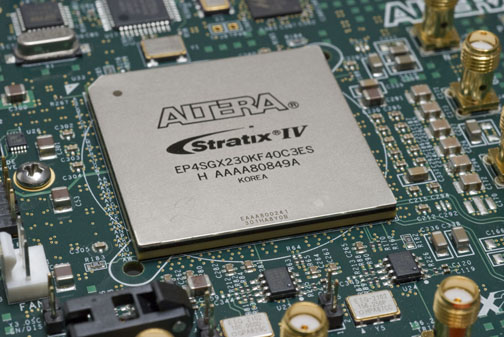
\includegraphics[width=1\linewidth]{fpga}
      \caption{Altera Corporation, CC BY 3.0}
    \end{figure}
  \end{columns}
\end{frame}

\begin{frame}
  \frametitle{Synthesis}
  \begin{itemize}
    \item Hardware Description Language (HDL)
      \begin{itemize}
        \item Verilog, VHDL, \textellipsis
      \end{itemize}
    \item High-Level Synthesis (HLS)
      \begin{itemize}
        \item C, Haskell, OpenCL, \textellipsis
      \end{itemize}
  \end{itemize}
\end{frame}

\subsection{OpenCL}

\begin{frame}
  \frametitle{OpenCL}
  \begin{columns}[c]
    \column{.55\textwidth}
    \begin{itemize}
      \item Framework for heterogeneous computing
      \item OpenCL C
        \begin{itemize}
          \item Annotations like \texttt{\_\_kernel}, \texttt{\_\_global}, \textellipsis
        \end{itemize}
    \end{itemize}
    \column{.45\textwidth}
    \begin{figure}
      \begin{mdframed}[backgroundcolor=white]
        
\includegraphics[width=1\linewidth]{opencl}
      \end{mdframed}
    \end{figure}
  \end{columns}
\end{frame}

\subsection{FM-index}

\begin{frame}
  \frametitle{String-searching algorithms}
  \begin{itemize}
    \item Used in e.g. bioinformatics
    \item Na\"ive algorithm is too slow
    \item Solution: substring index
  \end{itemize}
\end{frame}

\begin{frame}
  \frametitle{FM-index}
  \begin{columns}[c]
    \column{.55\textwidth}
    \begin{itemize}
      \item Query time of sublinear complexity
      \item Burrows-Wheeler transform
      \item Multiple datastructures
    \end{itemize}
    \column{.45\textwidth}
    \[ \texttt{abracadabra\$} \]
    \[ \downarrow \]
    \[ \texttt{ard\$rcaaaabb} \]
  \end{columns}
\end{frame}

\section{Thesis outline}
\begin{frame}
  \frametitle{Thesis outline}
  Analyzing performance of high-level synthesis \textellipsis

  \textellipsis by implementing FM-index in OpenCL as a case study
\end{frame}

\section{Experimental setup}

\begin{frame}
  \frametitle{Experimental setup}
  \begin{itemize}
    \item Measure throughput and energy consumption for 7500 search patterns
    \item Variable parameters:
      \begin{enumerate}
        \item Three corpora: DNA, proteins and XML
        \item Text sizes: 10, 14, 20 MB
        \item Search pattern sizes: 4, 6, 8 characters
      \end{enumerate}
  \end{itemize}
\end{frame}

\section{Implementations}

\subsection{Reference implementations}

\begin{frame}
  \frametitle{Reference implementations}
  \begin{itemize}
    \item Reference CPU application
    \item Reference FPGA application
      \begin{itemize}
        \item Only string-searching algorithm
        \item As close to CPU as possible
      \end{itemize}
  \end{itemize}
\end{frame}

\subsection{Optimized FPGA application}

\begin{frame}
  \frametitle{Optimized FPGA implementation}
  \begin{itemize}
    \item Paralellizing loop over patterns
    \item Caching \texttt{\_\_global} memory in \texttt{\_\_local} memory
    \item Burst memory transfers
  \end{itemize}
\end{frame}

\section{Results}

\begin{frame}
  \frametitle{Reference CPU results}
  \centering
  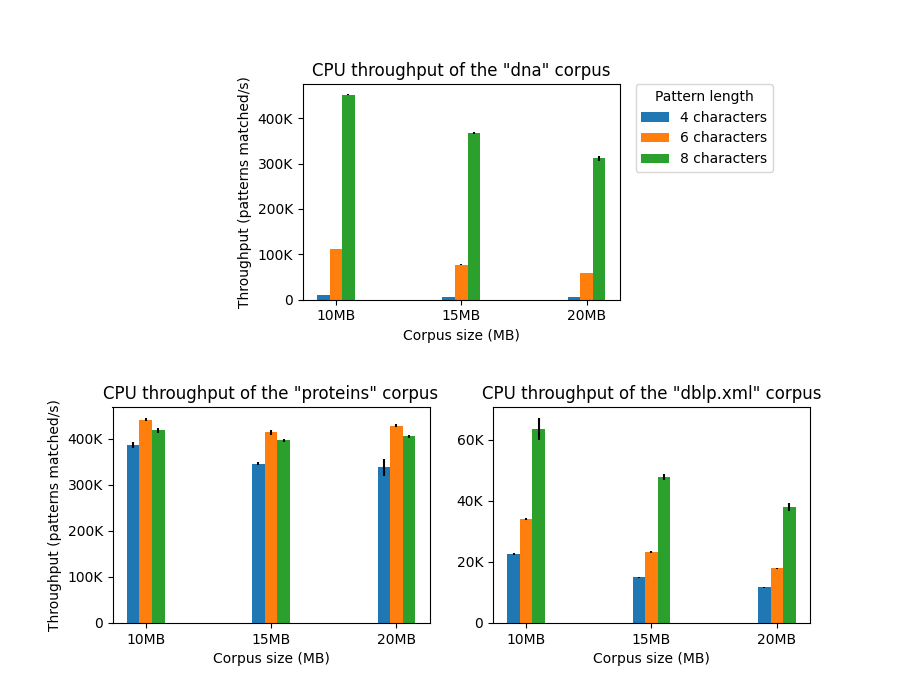
\includegraphics[width=0.67\linewidth]{throughput_cpu}
\end{frame}

\begin{frame}
  \frametitle{Speedup of reference FPGA application}
  \centering
  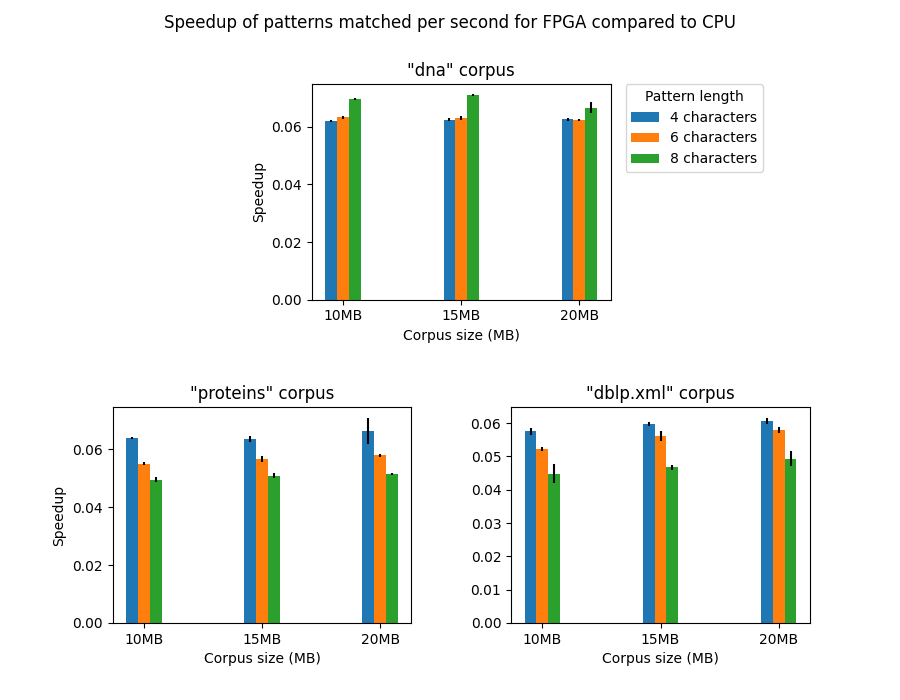
\includegraphics[width=0.67\linewidth]{speedup_fpga}
\end{frame}

\begin{frame}
  \centering
  Thank you for your attention!

  Any questions?
\end{frame}

\end{document}
